% Final report; original draft source and PDF are preserved in the parent directory.
\documentclass[conference,10pt]{IEEEtran}
\IEEEoverridecommandlockouts

\setlength{\tabcolsep}{3pt}
\usepackage{microtype}
\usepackage{cite}
\usepackage{amsmath,amssymb}
\usepackage{graphicx}
\usepackage{booktabs}
\usepackage{xcolor}
\usepackage{url}
\usepackage[hidelinks]{hyperref}

\graphicspath{{figures/}}

\newcommand{\lime}{LIME-$\Delta$}
% Float placement: allow figures/tables to sit in the text instead of piling up at page tops.
\renewcommand{\topfraction}{0.85}
\renewcommand{\textfraction}{0.15}
\renewcommand{\floatpagefraction}{0.75}
\setlength{\textfloatsep}{10pt plus 2pt minus 2pt}
\setlength{\intextsep}{10pt plus 2pt minus 2pt}

\begin{document}

\title{Can a Troubleshooter Trust a Filter Surrogate's Explanation?}

\author{\IEEEauthorblockN{Guohao Xiang; Ziyue Xiong; Mengyao Lee}
\IEEEauthorblockA{DSCI 498: Explainable AI, Lehigh University\\
Final report, Fall 2026}}

\maketitle

\begin{abstract}
We study whether explanations of a neural surrogate for a coupled-line microstrip band-pass filter can be trusted by a receive-side RF troubleshooter who must decide which failed specification to check and what to hand to the component designer.
The surrogate (PR-Net, a pole--residue network) is developed using a dataset of 1440 ADS circuit simulations with six geometry inputs and three negative-control inputs.
We explain a reference-relative (contrastive) mask-violation target with exact SHAP, Integrated Gradients and a LIME-based contribution, and ask three questions.
\emph{True:} on a test set frozen before evaluation, SHAP attributions agree with ground-truth Shapley values computed in ADS (Spearman 0.98--0.99, sign agreement 1.00), while IG and LIME differ through their attribution definitions and, for some targets, numerical or local-fit limitations.
\emph{Useful:} in a pre-registered tuning experiment, changing only the two SHAP-ranked parameters fixed 25 of 30 failing designs versus 6 of 30 for random pairs; however, a plain six-parameter surrogate search fixed all 30, supporting localization under a two-parameter restriction rather than a speed advantage over unrestricted optimization.
\emph{Hold up:} when three SHAP-tuned designs were re-simulated with an independent full-wave solver (openEMS), none passed the mask; two improved by about 13\,dB and one became worse.
Both full-wave baseline calculations give a narrower passband. In the three tuned openEMS cases, absolute $-3$\,dB bandwidth is 124--142\,MHz narrower, or 80--87\,MHz under a peak-relative definition; modeling and numerical differences remain possible contributors.
A trust heuristic from prior filter work, SHAP--LIME agreement, barely predicted agreement with ground truth (Spearman 0.24 over 3120 repeated model--design--target entries).
\end{abstract}

\begin{IEEEkeywords}
explainable AI, SHAP, integrated gradients, LIME, faithfulness, surrogate model, microstrip filter, full-wave validation
\end{IEEEkeywords}

%======================================================================
\section{Introduction}
%======================================================================
Neural surrogates approximate simulated microwave responses for rapid screening, and recent work has attached post-hoc explanations to them~\cite{suslova2026}.
Whether such explanations deserve trust depends on who uses them and for what decision.
Table~\ref{tab:frame} fixes the four elements of the project and the explanation principle, and the framing question follows from them:

\begin{quote}
\emph{For a receive-side RF troubleshooter deciding which failed specification and frequency region to check first and what to hand to the component designer, does an explanation built on the contrastive principle improve decision quality without losing faithfulness?}
\end{quote}

\begin{table}[htbp]
\centering
\caption{Project framework.}
\label{tab:frame}
\small
\begin{tabular}{p{0.20\linewidth}p{0.70\linewidth}}
\toprule
Data & 1440 ADS circuit simulations of a coupled-line microstrip band-pass filter; 6 geometry inputs + 3 planted negative controls; $S$-parameters 9--15\,GHz. \\
Model & PR-Net, a pole--residue neural surrogate (main); M1 black-box MLP and M0 (replication of~\cite{suslova2026}) as comparisons. \\
Stakeholder & Receive-side RF troubleshooting engineer (one practitioner, two interviews) and practitioner sources~\cite{rs_evm,adi_an1354}. \\
Decision & Which failed specification and frequency region to examine first; what to hand to the component designer (a ranked geometry hypothesis, not a validated fix). \\
Principle & Contrastive (Lipton~\cite{lipton1990}): why does this design violate the mask \emph{rather than} behave like a known-good reference design? \\
Improve / keep & Assess decision support through ADS-confirmed fixes under a two-parameter restriction (a proxy); keep faithfulness (to the model and to an ADS ground truth). \\
\bottomrule
\end{tabular}
\end{table}

We answer the three course questions with evidence of different strength:
(Q1) \emph{are the explanations true}---faithful to the model and to a simulator ground truth;
(Q2) \emph{are they useful}---measured by a pre-registered decision proxy and shaped by a practitioner interview;
(Q3) \emph{do they hold up}---when the circuit simulator that generated the training data is replaced by a full-wave electromagnetic solver.

\textbf{Contributions.}
(i) A ground-truth faithfulness test in which Shapley values are computed directly in the circuit simulator (64 coalitions per design) on a test set frozen before evaluation, allowing us to distinguish model-game mismatch from differences between attribution methods.
(ii) A pre-registered, simulator-confirmed tuning experiment that compares explanation-guided decisions with random, sensitivity-based, ground-truth and explanation-free baselines, including an unfavourable baseline.
(iii) A full-wave stress test showing that a decision validated inside the circuit model does not transfer, together with response-level evidence and an explicitly qualified account of the discrepancy.
(iv) A negative result for the SHAP--LIME agreement heuristic used in prior filter work~\cite{suslova2026}.

\textbf{What was written down before results.} Table~\ref{tab:prereg} lists each test, when its protocol or expectation was recorded, and the outcome. Where we could not prove that a protocol preceded its results, we say so.

\begin{table*}[!t]
\centering
\caption{Tests, the record written before results, and outcomes.}
\label{tab:prereg}
\small
\begin{tabular}{p{0.30\linewidth}p{0.30\linewidth}p{0.28\linewidth}}
\toprule
Test / expectation & Recorded before results & Outcome \\
\midrule
Negative controls: a model that ignores them should receive $\approx0$ attribution & Planted in the dataset; expectation in the analysis plan (Oct 24) & Supported (Sec.~\ref{sec:ground}) \\
Train-domain expectation: T0 ranking $L_2>L_1>W_{c2}$ & Analysis plan (Oct 24) & Supported by all methods \\
Explainer vs.\ ADS ground-truth Shapley; explainer/network/physics decomposition & Hash-frozen protocol, Oct 25 17:21 UTC, before any test label was read (no numeric threshold set) & SHAP 0.98--0.99; IG/LIME lower (Sec.~\ref{sec:truth}) \\
Explainer-selected parameter pairs fix more failing designs than random pairs & Pre-registration, Oct 25 19:23 UTC, before tuning code ran & Supported, $p_\text{Holm}=4\times10^{-5}$ (Sec.~\ref{sec:q2}) \\
Full-wave transfer of tuned designs & Case rule fixed in code before simulation; no expected outcome recorded & 0/3 pass (Sec.~\ref{sec:q3}) \\
Deletion/insertion vs.\ random orders & Described in the plan, but the pre-run version cannot be verified & Reported as supporting only \\
\bottomrule
\end{tabular}
\end{table*}

%======================================================================
\section{Related Work}
%======================================================================
\textbf{Attribution methods.} SHAP~\cite{lundberg2017} allocates a prediction difference by the Shapley value~\cite{shapley1953}; Integrated Gradients~\cite{sundararajan2017} integrates gradients along a path from a baseline; LIME~\cite{ribeiro2016} fits a local surrogate.
Our fixed-reference construction makes the comparison explicit~\cite{lipton1990,miller2019}; LIME is converted to a slope-times-displacement comparison while retaining its local-fit meaning.

\textbf{Evaluating faithfulness.} Deletion/insertion curves~\cite{petsiuk2018} and retrain-based removal~\cite{hooker2019} test whether high-attribution inputs matter to the model; randomization tests~\cite{adebayo2018} check that explanations depend on the model at all.
Jacovi and Goldberg~\cite{jacovi2020} separate faithfulness from plausibility; we additionally compare with a simulator-defined reference allocation, available because the deterministic circuit simulator permits exhaustive coalition evaluation.

\textbf{Explanations for microwave surrogates.} Suslova et al.~\cite{suslova2026} applied SHAP and LIME to neural models of microstrip filters and used SHAP--LIME agreement as evidence of reliable explanations; we replicate their network (M0) and test that heuristic against ground truth.
The gap between circuit and electromagnetic models is classical in microwave design and motivates space mapping~\cite{bandler1994}; we use it here as the ``unusual condition'' for Q3.

%======================================================================
\section{Stakeholder and Decision}
%======================================================================
Our stakeholder evidence consists of two online voice interviews with the same RF fault-analysis and troubleshooting engineer, on November~5 and November~21, 2026. The practitioner works on receive-side front-end evaluation and system-level diagnosis.
Both records are edited summaries, not verbatim transcripts. The project was introduced beforehand, and the follow-up discussed the tuning result; its method-specific comments therefore reflect that context.
The practitioner treats the filter as a constraint on what reaches the receiver and does not edit microstrip geometry.
Typical problems (excess EVM, sensitivity loss, adjacent-channel interference) are narrowed by checking passband flatness, band edges and out-of-band rejection, then confirmed by measurement.
Practitioner sources agree that filter loss and rejection are only some of many contributors to such receiver-level symptoms~\cite{rs_evm,adi_an1354}, which is why the explanation must start from the failed filter specification rather than from the symptom.

Three requirements emerged and directly shaped our explanation design:
\textbf{(A) Specification first}---show the frequency region, the failed specification and the violation magnitude, in engineering units, before any attribution; a bare ranking such as ``L2 is important'' is not actionable.
\textbf{(B) Case-level quality}---an aggregate correlation does not say whether \emph{this} explanation is reliable.
\textbf{(C) Action boundary}---separate diagnostic attribution from a proposed parameter change, which needs separate validation.
Requirement (C) is why we evaluate tuning (Q2) and full-wave transfer (Q3) separately from faithfulness (Q1).
The follow-up identified four anticipated benefits: narrowing candidate parameter pairs, rejecting infeasible directions earlier, making cross-team reasoning discussable, and calibrating engineering intuition through repeated verification. The engineer would accept a suggestion only if it agrees with measurement or ADS checks, carries adequate quality information, lies within their authority, and has affordable verification cost. Geometry edits remain the component engineer's responsibility. These are qualitative judgments from one person, not measured gains in time or decision accuracy.

%======================================================================
\section{Data and Surrogate Models}
%======================================================================
\textbf{Data.} The dataset contains 1440 third-order coupled-line microstrip band-pass filters simulated in Keysight ADS (circuit level; substrate $H=15$\,mil, $\varepsilon_r=3.78$, lossless, ideal conductors), with $S_{21}$ and $S_{11}$ at 601 points from 9 to 15\,GHz.
Inputs are six geometry parameters (resonator lengths $L_1,L_2$, gaps $S_1,S_2$, widths $W_{c1},W_{c2}$, in mil) and three \emph{negative controls}---random columns that the simulator never sees.
The split is by design: 1008 train, 216 validation, 216 test.
The specification mask (Fig.~\ref{fig:case}) requires, in the passband 11.6--12.4\,GHz, $|S_{21}|\ge-0.5$\,dB and $|S_{11}|\le-10$\,dB; in 9--10.8\,GHz $|S_{21}|\le-20$\,dB; and in 13.2--15\,GHz $|S_{21}|\le-15$\,dB.
The hard \emph{mask violation} $V$ is the sum of the four worst-case exceedances in dB; $V=0$ means pass.

\textbf{Models.}
PR-Net maps the nine inputs to five conjugate pole pairs plus residues and evaluates $S_{21}$ and $S_{11}$ as a closed-form rational function, so its poles can be checked against vector-fitting ground truth~\cite{gustavsen1999}.
M1 is a frequency-conditioned MLP with the same complex output and no structural prior.
M0 reproduces the fully connected network of~\cite{suslova2026} and serves as a deliberately weaker model.
Each is trained with three seeds. M0 is an architectural adaptation: widths and loss are project choices, outputs include $S_{11}$, and its ADS dataset differs from the paper's CST data. Published errors below are contextual rather than a controlled cross-study benchmark.
On the test set (Table~\ref{tab:acc}) PR-Net reaches 0.084\,dB $S_{21}$ MAE and 2.7\,MHz centre-frequency error. The distinct study in~\cite{suslova2026} reports 1.11\,dB and 18\,MHz.

\begin{table}[!t]
\centering
\caption{Saved test accuracy, mean of three seeds. Curve MAE: 216 designs; $f_0$/BW: 202 valid single-band designs, peak-relative $-3$ dB.}
\label{tab:acc}
\small
\begin{tabular}{lrrrr}
\toprule
Model & \shortstack{$S_{21}$ MAE\\(dB)} & \shortstack{$S_{11}$ MAE\\(dB)} & \shortstack{$f_0$ MAE\\(MHz)} & BW $R^2$ \\
\midrule
PR-Net & 0.084 & 0.078 & 2.73 & 0.910 \\
M1 & 0.021 & 0.025 & 0.37 & 1.000 \\
M0 & 0.266 & 0.811 & 29.3 & $-0.342$ \\
Prior study~\cite{suslova2026} & 1.11 & -- & 18 & $-1.28$ \\
\bottomrule
\end{tabular}
\end{table}

%======================================================================
\section{Explanations and the Contrastive Principle}
%======================================================================
\textbf{Targets.} Attributions explain scalar functions of the predicted response:
T0 (spectral centroid, a known-answer check), T1 (point values of $S_{21}$/$S_{11}$),
T1b (mean passband $S_{21}$, the target of~\cite{suslova2026}),
T2 (smoothed passband ripple, worst passband return loss and mask violation; our main object), and T3 (resonator pole frequencies and $Q$, PR-Net only).
The smooth mask violation uses a log-sum-exp with temperature 0.05\,dB.

\textbf{Contrastive principle.} Following Lipton~\cite{lipton1990} and Miller~\cite{miller2019}, we explain a \emph{contrast}: why design $x$ violates the mask by $V(x)$ \emph{rather than} behaving like a fixed reference design $r$ (the ADS baseline geometry, controls at train mean).
This supplies a stated reference and unit, as Requirement~A demands. Failed frequency regions are identified from the response and specification components; attribution of a single aggregate violation target does not itself localize the failure in frequency.

\textbf{Methods.}
\emph{SHAP}~\cite{lundberg2017,shapley1953}: exact Shapley values of the single-reference game $v(S)=f(x_S,r_{\bar S})$, enumerating all $2^9=512$ coalitions, so there is no sampling error.
\emph{IG}~\cite{sundararajan2017}: path integral of gradients from $r$ to $x$ (64 trapezoidal steps, increased to 128 and then 256 where the relative completeness residual exceeds 1\%).
\emph{LIME}~\cite{ribeiro2016}: local weighted linear fit around $x$; for comparison with additive methods we report \lime, the local slope times the displacement $x-r$, which is not an exact decomposition.
The methods answer different questions---reference-relative contribution, path-integrated sensitivity, local linear trend---so we expect principled disagreement on non-linear targets.
Reported Spearman scores compare attribution magnitudes; simulator sign agreement includes features whose ADS-reference magnitude is at least 1\% of target training standard deviation. Values displayed as 1.00 are rounded, not claims of exact agreement on every feature.

%======================================================================
\section{Q1: Are the Explanations True?}
%======================================================================
We separate two meanings of ``true''~\cite{jacovi2020}: faithful to the \emph{model}, and consistent with the \emph{simulator} that generated the data.

\subsection{Faithfulness to the model}
\label{sec:q1model}
\textbf{Internal checks.} SHAP additivity error is at most $1.6\times10^{-4}$.
IG completeness residual exceeds 1\% for 2.6\% of PR-Net entries overall but for 45\% of entries on the $S_{11}$ value at 12\,GHz, where the dB response passes near a log singularity; we treat this as a numerical failure mode, not a definitional disagreement.
LIME's held-out local $R^2$ has median 0.88 on T2, with 12\% of cases below 0.5.

\textbf{Deletion/insertion.} Following~\cite{petsiuk2018}, inputs are replaced by reference values in attribution order and the normalized area under the output curve is compared with 100 random orders.
On PR-Net T2 (40 validation designs), the SHAP order lies in the best 5\% of random orders for 80\% (deletion) and 89\% (insertion) of entries; IG 69\%/86\%; \lime{} 64\%/93\%.
With only nine, strongly ranked inputs this is an easy test, and we could not verify that its protocol was written before it was run, so we report it as supporting, not decisive, evidence.

\textbf{Negative controls.} With SHAP and IG, PR-Net assigns at most 1\% of total $|\phi|$ to the three controls (\lime: up to 4\%), matching its measured interventional sensitivity to them (0--1\%).
M0 assigns 3--7\% (SHAP), consistent with its actual sensitivity of 4--8\%: the explanation correctly exposes that the weaker model uses a spurious input~\cite{adebayo2018}.

\subsection{Where and why the three methods disagree}
\label{sec:disagree}
On PR-Net (validation, rank correlation of $|\phi|$ over nine inputs) the methods agree almost perfectly on the near-linear known-answer target T0 (SHAP--IG 0.99, SHAP--\lime{} 0.96) and diverge on the non-linear mask target T2 (0.93 and 0.85); a linear model explains only 13--23\% of the variance of the T2 targets.
We trace the disagreement to four sources:
\begin{enumerate}
\item \emph{Different questions.} SHAP averages marginal effects over all coalitions with the reference; IG follows one straight path; \lime{} extrapolates a local slope over the whole displacement. With interactions (e.g.\ between $L_1$ and $L_2$, which jointly set band position) these are different quantities, not noisy estimates of one.
\item \emph{Numerics.} IG violates completeness near $S_{11}$ notches (Sec.~\ref{sec:q1model}), where the dB target is nearly singular.
\item \emph{Locality.} Halving LIME's neighbourhood (0.5$\to$0.25) changes its T2 ranking (0.85), and a new sampling seed changes it further (0.91).
\item \emph{Reference.} SHAP with one reference vs.\ a 32-design background agrees only at 0.70--0.78; the ``contrast'' changes, so the answer changes.
\end{enumerate}
The simulator comparison in Sec.~\ref{sec:truth} tests agreement with the chosen Shapley allocation. Its definition favors a matching Shapley estimator; it does not turn every path or local-fit difference into a failure of faithfulness.

\subsection{Domain grounding: what the model should have learned}
\label{sec:ground}
We distinguish exact simulator invariance, train-domain expectations and concept checks.
(i) \emph{Controls:} the simulator never reads the three control columns, so their true effect is exactly zero; PR-Net's explanations reflect this (above).
(ii) \emph{Train-domain expectation:} prior train-side analysis suggested that resonator lengths dominate T0, with ranking $L_2>L_1>W_{c2}\gg$ others. All four methods (SHAP, IG, LIME slope, gradient) recover it on PR-Net (rank correlation 0.94 with train regression). The precise order is empirical for this dataset, not a universal physical law.
(iii) \emph{Filter physics:} resonator length should dominate band position and coupling gap should shape the response; the ADS ground truth for the mask violation ranks $L_2>L_1>S_2$ on both splits, and for the quality factor of the middle in-band pole it ranks coupling geometry first ($S_1>W_{c1}$), as expected for a coupling-controlled quantity.
(iv) \emph{Concepts:} PR-Net's internal pole frequencies and $Q$ (T3) can be checked against vector fitting~\cite{gustavsen1999} of the ADS responses; the model's finite-difference sensitivities of these concepts match the vector-fitted ADS ones (sign agreement 0.98, rank correlation 0.99), and SHAP on T3 matches the ADS Shapley values at 0.98. These are fitted modal concepts, not independently measured resonator parameters.

\subsection{Consistency with a simulator ground truth}
\label{sec:truth}
\textbf{Protocol written before evaluation.} On October~25, 2026 (17:21 UTC), the project recorded SHA-256 hashes of 30 files with a protocol and a statement that no test labels had yet been read (Table~\ref{tab:prereg}); validation had already informed development. The loader gates explicit label access on that record's existence. The current audit matches 26 hashes, including all nine neural weights. Four evolving plan/protocol or test-path files differ; the plan documents these changes, but original snapshots were not reconstructed. This is a local record, not an independently timestamped public registration.
For 80 designs (40 validation, 40 test) we simulated all $2^6=64$ geometry coalitions of the same single-reference game directly in ADS, giving exact ground-truth Shapley values for every target.
The full coalition reproduces the dataset exactly (max $|\Delta S|=0$).

\textbf{Result.} Fig.~\ref{fig:decomp} decomposes agreement into \emph{network vs.\ ADS} (does the model's own game match physics?) and \emph{explainer vs.\ ADS}.
For PR-Net the network game agrees with ADS at Spearman 0.98--0.99 on every target; SHAP inherits this (0.98--0.99, sign agreement 1.00), while IG falls to 0.82 and \lime{} to 0.84 on T2.
This supports simulator consistency of the surrogate's reference game. The remaining IG/LIME difference includes different estimands as well as numerical and local-fit effects; it cannot all be called explainer error.
For M0 the network itself agrees with ADS at only 0.80--0.91; SHAP tracks the network (0.81--0.92), while IG and \lime{} lose up to a further 0.05.
A naive explanation from train-set linear regression reaches only 0.56--0.59 on T1b/T2, so the model-based explanations add real information.

\begin{figure}[htbp]
\centering
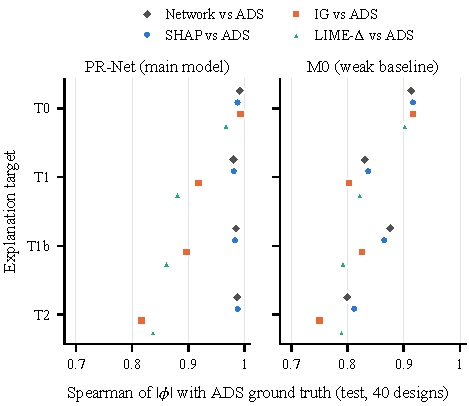
\includegraphics[width=\linewidth]{fig_decomposition.pdf}
\caption{Agreement of attribution magnitudes with ADS ground-truth Shapley values (test). ``Network vs ADS'' compares the model game with the simulator. Other points compare method allocations with that Shapley reference, combining definition and approximation differences.}
\label{fig:decomp}
\end{figure}

\textbf{A trust heuristic that fails.} Prior work~\cite{suslova2026} reads SHAP--LIME rank agreement as a sign of trustworthy explanations.
Across 3120 model--design--target entries from 80 designs, this agreement is associated with ADS-reference agreement at Spearman 0.24 (0.20--0.24 per model under the original protocol; 0.12--0.15 for PR-Net and M1, 0.47 for M0, when SHAP and \lime{} use the same single-reference game as the ground truth).
These repeated entries are not independent cases. Agreement between explainers is weak evidence of ADS-reference agreement in this setup and is not calibrated as a single-case trust score.

%======================================================================
\section{Q2: Are the Explanations Useful?}
\label{sec:q2}
%======================================================================
We have no user study; Q2 rests on a decision proxy and on the interview.
The proxy models Requirement~C's hand-off: if an attribution selects two parameters contributing to reference-relative model violation, does a search restricted to them find an ADS-confirmed pass?

\textbf{Pre-registered experiment.} Before running any tuning code we wrote down cases, selectors, search and statistics with a UTC timestamp and plan hash.
Thirty failing single-band test designs were drawn with a fixed seed.
Each selector picks two of the six geometry parameters; a PR-Net search inside that two-dimensional box (41$\times$41 grid plus projected Adam, objective = smooth violation with a safety margin + a small move penalty) proposes a design, and ADS confirms it.
Up to ten ADS calls are allowed per case, the margin growing by 0.25\,dB after each failed call; success means ADS hard violation $V=0$.
The primary test is exact McNemar of each explainer versus random pairs, Holm-corrected.

\begin{figure*}[!t]
\centering
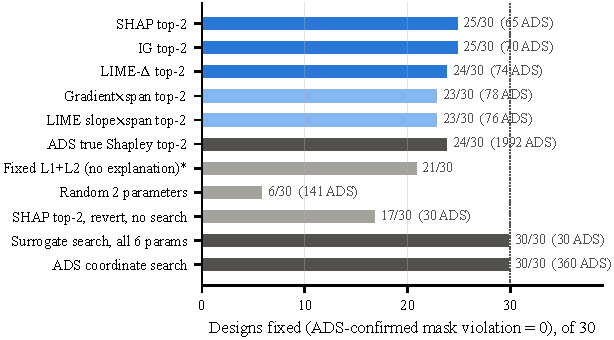
\includegraphics[width=0.80\linewidth]{fig_tuning.pdf}
\caption{Pre-registered tuning on 30 failing test designs (PR-Net surrogate, ADS confirmation). Blue: explanation-selected pairs; light blue: sensitivity baselines; dark: references; gray: baselines. Totals in brackets are ADS calls (ground-truth Shapley includes 64 coalition simulations per case). *Exploratory, not pre-registered.}
\label{fig:tuning}
\end{figure*}

\textbf{Result} (Fig.~\ref{fig:tuning}).
SHAP-selected pairs fixed 25/30 designs versus 6/30 for random pairs (20 vs.\ 1 discordant cases, McNemar $p_{\text{Holm}}=4.2\times10^{-5}$; median paired reduction of the best ADS violation versus random 4.5\,dB, Wilcoxon $p_{\text{Holm}}=4.2\times10^{-5}$); IG 25/30 and \lime{} 24/30 were equally significant.
SHAP chose the same pair as the ADS ground truth in 87\% of cases at 1/30 of the simulation cost.
Two baselines temper this result.
A six-parameter surrogate search \emph{without any explanation} fixed all 30 designs with a single ADS call each, and always tuning $L_1$+$L_2$ fixed 21/30.
Reverting the SHAP-top-2 parameters to the reference without searching fixed only 17/30: the explanation names \emph{where} to act but not \emph{how much}.
In an exploratory rerun with the weaker M0 as surrogate, SHAP still fixed 22/30, providing a second, exploratory model comparison rather than a general model-quality scaling law.

\textbf{Interpretation for the stakeholder.} The experiment does not show a tuning-speed advantage over all-parameter optimization. It supports localization under a two-parameter restriction. The interviews additionally motivate communication and screening benefits, conditional on independent checks and role-appropriate actions; these human benefits were not measured.
Table~\ref{tab:card} shows the case summary we propose, ordered by Requirements A--C.
The November~21 follow-up supplies qualitative workflow feedback. It does not document operation of this particular case card or demonstrate improved task performance. The engineer's four-benefit account is retained as a design motivation, including the objection that aggregate agreement cannot certify one design.

\begin{table*}[!t]
\centering
\caption{Specification-first case card for test\_0005. Diagnostics concern the smooth mask target, PR-Net seed 2026; quality indicators have distinct meanings.}
\label{tab:card}
\small
\begin{tabular}{p{0.14\linewidth}p{0.80\linewidth}}
\toprule
A Failure & Passband 11.6--12.4 GHz: $S_{11}$ exceeds $-10$ dB by 6.1 dB and $S_{21}$ falls below $-0.5$ dB by 1.8 dB; hard total $V=7.9$ dB. Stopbands pass. \\
B Prediction & Same-target smooth violation error against ADS at this design: 0.0749 dB. This is a checked retrospective error, not a predictive uncertainty interval. \\
B Explanation & SHAP additivity error $3.24\times10^{-8}$; IG relative completeness residual 0.0821\% at 64 steps; LIME held-out local $R^2=0.846$ (neighborhood 0.25, seed 0). These checks do not certify hardware correctness. \\
C Diagnosis & Relative to the reference, SHAP ranks $L_1$ and $S_2$ highest for mask violation. Frequency context comes from the response checks above. \\
C Proposal & Change $L_1$ by +7.2 mil and $S_2$ by +0.6 mil: passes in ADS circuit simulation, but fails the mask by 10.2 dB in openEMS. A troubleshooting engineer can request checks or a designer review; geometry changes need separate authority and validation. \\
\bottomrule
\end{tabular}
\end{table*}

%======================================================================
\section{Q3: Do the Decisions Hold Up Under a Change of Physics Model?}
\label{sec:q3}
%======================================================================
The ADS labels evaluate an interconnected network of distributed coupled-line elements. openEMS is a three-dimensional full-wave solver using EC-FDTD, which advances a spatially discretized electromagnetic solution in time~\cite{openems_docs}. ``Equivalent circuit'' describes that field-discretization formulation; it does not make it the same component-level model as ADS. Momentum supplies a frequency-domain method-of-moments full-wave solution for planar conductors in a layered substrate~\cite{keysight_momentum}. These different formulations provide a cross-check, while ports, boundaries, discretization and physical assumptions can also influence differences. Unlike the below-6-GHz scope of~\cite{suslova2026}, this dataset is near 12 GHz; frequency alone is not isolated as the cause of failure.
We originally planned a few HFSS checks; without a licence we used the open-source FDTD solver openEMS~\cite{liebig2013} (v0.37) on the identical layout as the dataset's Momentum diagnostic template (zero-thickness PEC, same lossless substrate, 50\,$\Omega$ microstrip ports, 601 frequency points).

\textbf{Calibration.} Mesh refinement on the baseline (Fig.~\ref{fig:mesh}) moves the openEMS centre frequency \emph{up} (11.89$\to$12.03\,GHz; last step 22\,MHz) while Momentum moves \emph{down} (12.18$\to$12.13\,GHz), bracketing the ADS value of 12.05\,GHz.
The mesh sensitivity limits interpretation of the original Momentum--circuit offset; opposite refinement trends do not establish a shared limit or prove the circuit value is correct.
Using absolute $-3$\,dB edges, baseline bandwidths are openEMS 1.163, Momentum 1.131 and ADS 1.287\,GHz; using peak-relative edges, they are 1.209, 1.143 and 1.287\,GHz. Both comparisons show narrowing, with different magnitudes. About 17--18\% of baseline passband power is not returned through the two recorded ports ($1-|S_{11}|^2-|S_{21}|^2$; ADS approximately zero). This is consistent with omitted full-wave loss mechanisms including radiation, but does not isolate radiation from numerical or port effects.
The finest openEMS mesh (3.8\,M cells, about 13\,min per run) was used for all cases.

\textbf{Case rule.} Walking the 30 pre-registered cases in order, we kept those where SHAP tuning succeeded in ADS and whose SHAP pair had not been used, stopping at three (test\_0005: $L_1,S_2$; test\_0015: $L_1,L_2$; test\_0034: $L_2,S_1$).
The rule was fixed in code before any case was simulated, but was not externally time-stamped.
Each original design $x_0$ and its SHAP-tuned design were simulated.

\textbf{Result.} None of the three tuned designs passes in full-wave (Fig.~\ref{fig:fw}, Table~\ref{tab:fw}).
For test\_0015 and test\_0034 the decision \emph{direction} transfers: violation drops by 13.5 and 13.4\,dB.
For test\_0005 it reverses: violation rises from 6.4 to 10.2\,dB.
The 5.0--10.2 dB final violations are large compared with the baseline's last refinement change of 0.12 dB. This is supporting sensitivity evidence; the six case geometries were not each subjected to their own mesh-convergence study.

\begin{figure*}[!t]
\centering
\begin{minipage}[t]{0.48\linewidth}
\centering
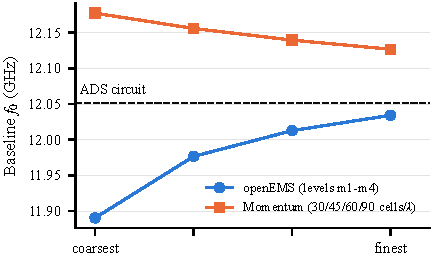
\includegraphics[width=\linewidth]{fig_mesh.pdf}
\caption{Baseline centre frequency under mesh refinement. The full-wave estimates move in opposite directions with refinement; a common converged value is not established. Here $f_0$ uses absolute $-3$ dB edge midpoints.}
\label{fig:mesh}
\end{minipage}\hfill
\begin{minipage}[t]{0.48\linewidth}
\centering
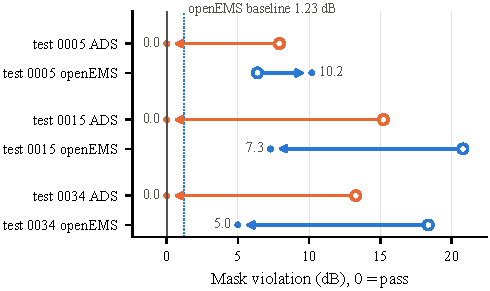
\includegraphics[width=\linewidth]{fig_fullwave_summary.pdf}
\caption{Mask violation before (hollow) and after (filled) SHAP-guided tuning, in ADS and in openEMS. Dotted: untouched baseline in openEMS.}
\label{fig:fw}
\end{minipage}
\end{figure*}

\begin{table*}[!t]
\centering
\caption{Paired full-wave checks at openEMS mesh m4. Frequency shift and the first BW shift use absolute $-3$ dB edges; the last column uses peak-relative edges. All shifts are openEMS minus ADS for the tuned design.}
\label{tab:fw}
\small
\begin{tabular}{lrrrrrr}
\toprule
Design & \shortstack{ADS $V$ dB\\$x_0\to$tuned} & \shortstack{openEMS $V$ dB\\$x_0$} & \shortstack{openEMS $V$ dB\\tuned} & \shortstack{$f_0$ shift\\MHz} & \shortstack{Absolute BW shift\\MHz} & \shortstack{Relative BW shift\\MHz} \\
\midrule
test\_0005 & $7.9\to0$ & 6.4 & 10.2 & $-49$ & $-124$ & $-80.1$ \\
test\_0015 & $15.2\to0$ & 20.8 & 7.3 & $-49$ & $-129$ & $-82.3$ \\
test\_0034 & $13.3\to0$ & 18.4 & 5.0 & $-53$ & $-142$ & $-86.9$ \\
\bottomrule
\end{tabular}
\end{table*}

\textbf{Mechanism.} The preregistered search stops at the first ADS pass and does not require a margin calibrated for the full-wave discrepancy.
For these tuned designs, absolute bandwidth is 124--142 MHz narrower and its edge midpoint is about 50 MHz lower; peak-relative bandwidth shrinks by 80--87 MHz. The paired responses show passband $S_{21}$/$S_{11}$ and low-stopband violations, with no high-stopband violation. The data support a model-discrepancy explanation, but do not uniquely assign each change to one physical mechanism.
test\_0005 (Fig.~\ref{fig:case}) is instructive: its original failure was matching ($S_{11}$), with a well-centred passband (12.05\,GHz).
The SHAP pair $L_1,S_2$ repaired it in ADS by moving the centre frequency down 141\,MHz---a path that is valid in the circuit model but runs in the same direction as the circuit-to-full-wave shift, adding a 3.3\,dB low-stopband violation in full-wave.
The attribution was faithful to the model it explained; the \emph{decision} built on it inherited that model's systematic error.

\begin{figure*}[!t]
\centering
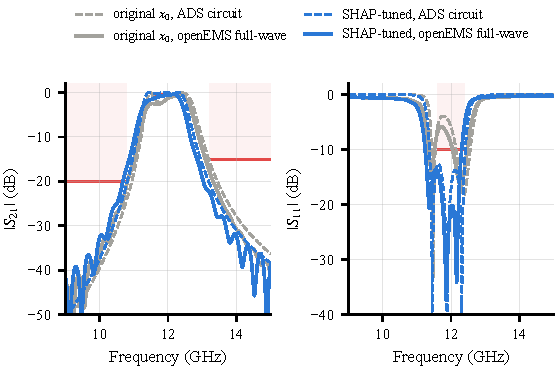
\includegraphics[width=0.80\linewidth]{fig_fullwave_case.pdf}
\caption{test\_0005 before (gray) and after (blue) SHAP-guided tuning; dashed: ADS circuit, solid: openEMS full-wave. Red segments: mask limits; shaded: forbidden regions. The tuned design passes in ADS but moves into the low stopband in full-wave.}
\label{fig:case}
\end{figure*}

%======================================================================
\section{Failed or Abandoned Explanations}
%======================================================================
\begin{itemize}
\item \textbf{SHAP--LIME agreement as a trust signal} (Sec.~\ref{sec:truth}): barely predicts ground-truth agreement (Spearman 0.24 overall). Abandoned as a quality indicator for Requirement~B.
\item \textbf{IG on $S_{11}$ notches}: 45\% of entries violate completeness by more than 1\% even with 256 steps. The proposed presentation therefore flags or withholds such IG results rather than treating them as reliable.
\item \textbf{SHAP read as local sensitivity}: at the baseline, SHAP magnitudes (distributional background) agree with ADS single-parameter perturbations at Spearman only 0.33, whereas gradient$\times$span reaches 0.58 and model finite differences 0.98. SHAP answers a contrastive question, not ``which knob is most sensitive here''.
\item \textbf{Background dependence}: single-reference SHAP and SHAP with a 32-point background agree only at 0.70--0.78; the reference must always be stated.
\item \textbf{Attribution as a step size}: reverting the top-2 SHAP parameters to the reference fixed only 17/30 designs.
\item \textbf{Tuning advice across models}: 0/3 SHAP-tuned designs pass in full-wave (Sec.~\ref{sec:q3}).
\item \textbf{Abandoned framing}: we first framed the stakeholder as a filter designer choosing which two dimensions to tune. The only practitioner available does not edit geometry, so the decision was re-framed to troubleshooting and hand-off.
\end{itemize}

%======================================================================
\section{Limitations}
%======================================================================
Stakeholder evidence is two paraphrased interviews with one practitioner; Q2 is a simulator proxy, not a user study.
The full-wave check covers three designs and shows a clear counter-example with a consistent mechanism, not a failure rate.
openEMS is not HFSS and shows extra non-physical loss out of band (12\% at 9\,GHz versus 2\% for Momentum), visible as ripple below $-30$\,dB; the recorded hard-mask violations persist in the checked responses, but boundary/port sensitivity has not been fully isolated.
The compared setups assume ideal conductors and a lossless substrate. Finite-conductivity, material and manufacturing effects and fabricated-device measurements remain outside this study.
The reference Shapley game is defined for one baseline; others can rank parameters differently. The nine-input model explanation includes controls that are absent from the six-geometry ADS game. Quality diagnostics such as local $R^2$ and completeness do not give calibrated per-design probabilities of correctness.

%======================================================================
\section{Conclusion}
%======================================================================
For the troubleshooter's decision, the answer to our framing question is split.
The contrastive SHAP explanation closely recovers the selected network and ADS reference allocations. Method-definition differences and numerical failures must be distinguished when evaluating IG and LIME.
Its demonstrated utility is restricted-parameter localization in a simulator experiment; the interviews motivate a ranked hypothesis for designer handoff, without measured human decision gains or a tuning-speed advantage.
It does \emph{not hold up} as tuning advice when the physics changes: a design that the explanation helped to fix in the circuit model failed in full-wave in all three cases checked, and got worse in one.
The practical rule we would give the stakeholder is therefore Requirement~C made concrete: treat attribution as diagnosis, and independently validate any proposed change using the applicable physical model or measurement. The observed shifts motivate a margin study, not a generally certified 0.13 GHz/50 MHz safety rule.

\textbf{Code and records.} The repository is \url{https://github.com/gux225-spec/DSCI498_Project-for-xAI}. Its README explains source/evidence separation and reproduction; \texttt{docs/decision\_log.md} records decisions with timing qualifications. A new archived-result verifier checks the saved calculations without changing historical experiment files. The separate AI-use reflection describes AI-assisted ADS automation, technical-source interpretation and independent verification.

\bibliographystyle{IEEEtran}
\bibliography{references}

\end{document}
